\section*{Introduction}
Ce rapport détaille le processus de configuration d'un compilateur croisé pour Raspberry Pi 3 (architecture aarch64) en utilisant Crosstool-NG, ainsi que la configuration de l'environnement pour l'utilisation du compilateur et la configuration de QEMU pour l'exécution de programmes compilés.
Crosstool-NG : Crosstool-NG est un outil de construction de chaînes de compilation croisée. Il est utilisé pour générer des outils de développement tels qu'un compilateur, un linker et d'autres utilitaires, spécifiquement conçus pour une architecture cible différente de celle du système de développement. Dans notre cas, nous utilisons Crosstool-NG pour construire un compilateur croisé pour l'architecture aarch64 (Raspberry Pi 3).
\section{Mise à jour du système }
Tout d'abord, nous avons mis à jour la liste des paquets disponibles et effectué une mise à niveau du système à l'aide des commandes suivantes :
\begin{itemize}
    \item sudo apt update
     \item sudo apt dist-upgrade
\end{itemize}
\section{Installation des dépendances}
Nous avons installé les dépendances nécessaires à la compilation en utilisant la commande :
\\sudo apt install build-essential git autoconf bison flex texinfo help2man gawk libtool-bin libncurses5-dev unzip 


\section{Clonage de Crosstool-NG }
Nous avons cloné le référentiel Crosstool-NG depuis GitHub en utilisant la commande :
\\git clone https://github.com/crosstool-ng/crosstool-ng 
\begin{figure}[h]
    \centering
    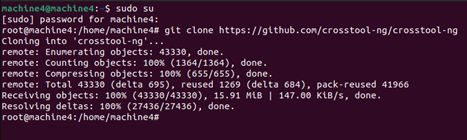
\includegraphics[width=1\textwidth]{images/8.png}
    
\end{figure}
\section{Accès au répertoire Crosstool-NG }
Nous nous sommes déplacés vers le répertoire nouvellement créé avec la commande :
\\cd crosstool-ng/ 
\begin{figure}[h]
    \centering
    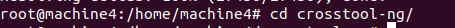
\includegraphics[width=1\textwidth]{images/9.png}
    
\end{figure}

\section{Bootstrap de Crosstool-NG }
Pour préparer l'environnement de compilation, nous avons exécuté la commande :
\\ ./bootstrap 
\section{Configuration de Crosstool-NG avec l'option --enable-local }
Nous avons configuré Crosstool-NG avec l'option --enable-local en utilisant la commande :
\\ ./configure --enable-local 
\begin{figure}[h]
    
    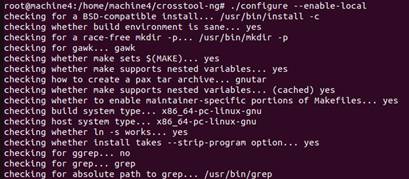
\includegraphics[width=1\textwidth]{images/10.png}   
\end{figure}
./configure --enable-local : La commande ./configure est couramment utilisée pour configurer un projet logiciel avant la compilation. Dans le cas de Crosstool-NG, ./configure --enable-local est utilisé pour configurer Crosstool-NG avec l'option --enable-local, qui indique à Crosstool-NG de construire la chaîne de compilation croisée localement, sur votre système. Cela signifie que la chaîne de compilation croisée sera générée sur votre système au lieu d'être téléchargée depuis des sources préconstruites.

\section{Compilation de Crosstool-NG }
Nous avons utilisé la commande \textbf{make} pour réellement construire Crosstool-NG, c'est-à-dire pour générer les outils de développement pour l'architecture cible.
\\Make est une commande de construction couramment utilisée dans les projets logiciels. Lorsqu'elle est exécutée, elle utilise un fichier Makefile pour compiler et assembler le code source du projet. 
\newpage
Dans le contexte de Crosstool-NG, make est utilisé pour réellement construire la chaîne de compilation croisée, c'est-à-dire pour générer les outils de développement pour l'architecture cible.
\begin{figure}[h]
    
    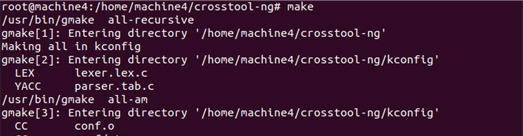
\includegraphics[width=1\textwidth]{images/11.png}   
\end{figure}

\section{Configuration de Crosstool-NG à l'aide de configurations prédéfinies}
Nous avons utilisé les configurations prédéfinies disponibles en utilisant la commande :

\textbf{./ct-ng list-samples }

\\ ./ct-ng list-samples est une commande qui liste les configurations prédéfinies (samples) disponibles pour Crosstool-NG. Ces configurations prédéfinies sont des ensembles de paramètres préconfigurés pour différentes architectures cibles. En utilisant cette commande, vous pouvez voir la liste des configurations prêtes à l'emploi pour choisir celle qui correspond à votre architecture cible.
\begin{figure}[h]
    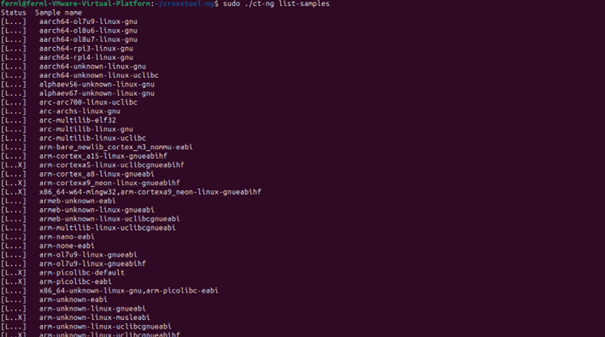
\includegraphics[width=1\textwidth]{images/12.png}   
\end{figure}

\section{Choix de la configuration prédéfinie }
Nous avons choisi la configuration prédéfinie pour l'architecture aarch64-rpi3-linux-gnu en utilisant la commande :
\\ ./ct-ng aarch64-rpi3-linux-gnu 
\newpage
\begin{figure}[h]
    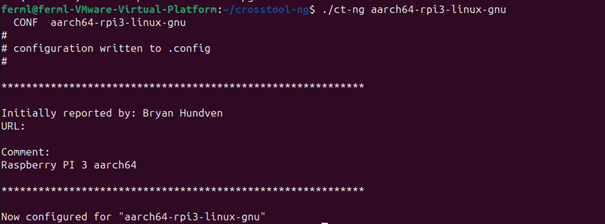
\includegraphics[width=1\textwidth]{images/13.png}   
\end{figure}
On peut utiliser ./ct-ng menuconfig pour configurer manuellement.  
\begin{figure}[h]
    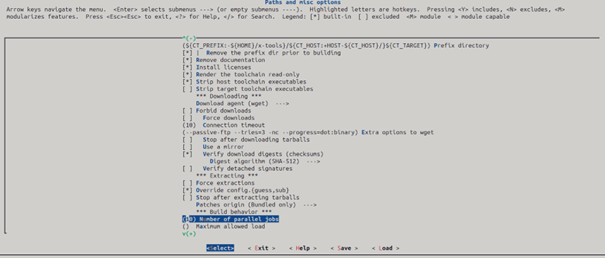
\includegraphics[width=1\textwidth]{images/14.png}   
\end{figure}
\section{Compilation du compilateur croisé}
 Nous avons lancé le processus de compilation du compilateur croisé en utilisant la commande :
\\ ./ct-ng build
\begin{figure}[h]
    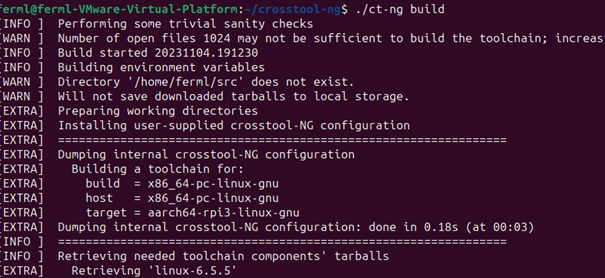
\includegraphics[width=1\textwidth]{images/15.png}   
\end{figure}

\section{Configuration de la variable PATH }
Nous avons configuré la variable PATH pour inclure le chemin du répertoire de notre compilateur croisé, tout en tenant compte de la configuration de LD\_LIBRARY\_PATH.
 Trouvez le chemin du répertoire où votre compilateur croisé a été installé. # Ajoutez le chemin du répertoire de votre compilateur croisé à la variable PATH en utilisant la commande suivante :
\begin{figure}[h]
    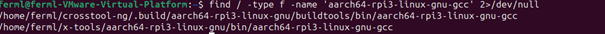
\includegraphics[width=1\textwidth]{images/16.png}   
\end{figure}

 \\export PATH=PATH:/home/ferml/x-tools/aarch64-rpi3-linux-gnu/bin
\begin{figure}[h]
    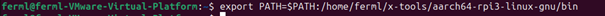
\includegraphics[width=1\textwidth]{images/17.png}   
\end{figure}

\section{Configuration de la variable CROSS\_COMPILE}
 Nous avons configuré la variable CROSS\_COMPILE dans les scripts de construction ou les fichiers de configuration pour spécifier le préfixe du compilateur croisé.
Trouvez le chemin du répertoire où votre compilateur croisé a été installé. # Configurez la variable CROSS\_COMPILE pour qu'elle corresponde au préfixe de votre compilateur croisé. export CROSS\_COMPILE=aarch64-rpi3-linux-gnu- 

\begin{figure}[h]
    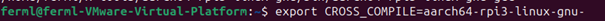
\includegraphics[width=1\textwidth]{images/19.png}   
\end{figure}
\section{Compilation d'un Programme de Test }
Une fois que vous avez créé avec succès la chaîne de compilation croisée avec Crosstool-NG, vous pouvez compiler un programme de test pour vérifier que le compilateur croisé fonctionne correctement. Assurez-vous d'avoir un fichier source, par exemple, testcompilation.c, que vous souhaitez compiler pour votre architecture cible.
\\Compilez le programme de test en utilisant le compilateur croisé que vous avez créé. Utilisez la commande aarch64-rpi3-linux-gnu-gcc (ou le préfixe approprié pour votre chaîne de compilation) pour compiler le programme. Par exemple :
\\aarch64-rpi3-linux-gnu-gcc -o testcompilation testcompilation.c 

\\Assurez-vous que testcompilation.c est le nom de votre fichier source et que vous spécifiez le nom de sortie (dans cet exemple, testcompilation).
\\Cette étape générera un exécutable pour votre architecture cible. 
\begin{figure}[h]
    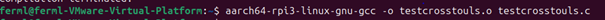
\includegraphics[width=1\textwidth]{images/20.png}   
\end{figure}

\section{Configuration de la variable LD\_LIBRARY\_PATH }
Nous avons configuré la variable LD\_LIBRARY\_PATH pour inclure le chemin des bibliothèques de notre compilateur croisé.
\\Configurez la variable LD\_LIBRARY\_PATH pour inclure 
\\le chemin des bibliothèques de votre compilateur croisé. 
\textbf{export LD\_LIBRARY\_PATH=/home/ferml/x-tools/aarch64-rpi3-linux-gnu/aarch64-rpi3-linux-gnu/sysroot/lib}


\section{Création d'un lien symbolique pour ld-linux-aarch64.so.1}
 Nous avons créé un lien symbolique pour `ld-linux-aarch64.so.1` pour assurer que le système cible peut trouver le linker dynamique nécessaire. ```bash # Créez un lien symbolique pour ld-linux-aarch64.so.1 dans le répertoire /lib du système. 
 \textbf{sudo ln -sf /home/ferml/x-tools/aarch64-rpi3-linux-gnu/aarch64-rpi3-linux-gnu/sysroot/lib/ld-linux-aarch64.so.1 /lib/ld-linux-aarch64.so.1 }
 \begin{figure}[h]
    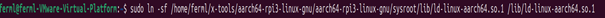
\includegraphics[width=1\textwidth]{images/21.png}   
\end{figure}
\section{Configuration de QEMU }
Pour exécuter des programmes compilés avec le compilateur croisé, nous avons configuré QEMU.
ferml@ferml-VMware-Virtual-Platform:~ aarch64-rpi3-linux-gnu-gcc -o testcompilation testcompilation.c
 \begin{figure}[h]
    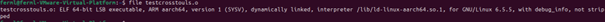
\includegraphics[width=1\textwidth]{images/22.png}   
\end{figure}
\\•	Assurez-vous que QEMU est installé avec la commande sudo apt install qemu.
\\•	Utilisez la commande qemu-aarch64 pour spécifier l'architecture cible.
 \begin{figure}[h]
    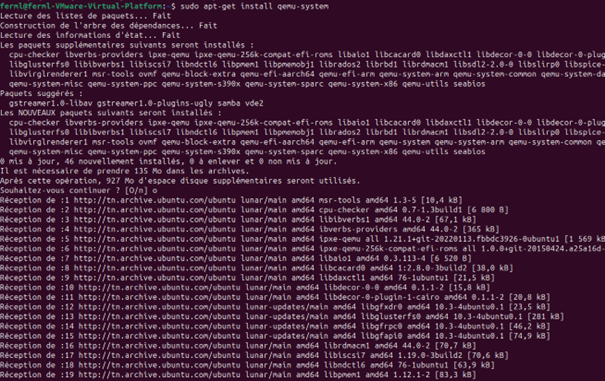
\includegraphics[width=1\textwidth]{images/23.png}   
\end{figure}
\newpage
\\ferml@ferml-VMware-Virtual-Platform:~ qemu-aarch64 ./testcompilation Hello, World!
 \begin{figure}[h]
    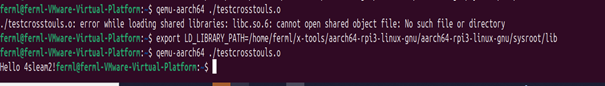
\includegraphics[width=1\textwidth]{images/24.png}   
\end{figure}

\section*{Conclusion}

En conclusion, ces étapes sont cruciales pour assurer le bon fonctionnement des programmes compilés avec le compilateur croisé sur le système cible, en particulier le Raspberry Pi 3. La configuration actuelle du système est désormais optimale pour le développement et les tests de logiciels spécifiquement adaptés à cette plateforme.